\documentclass[pdflatex,sn-basic]{sn-jnl}

\usepackage{graphicx}
\usepackage{amsmath,amssymb}
\usepackage{booktabs}
\usepackage{url}

\raggedbottom

\newcommand{\TaskCount}{60}
\newcommand{\CandidateCount}{300}
\newcommand{\KilledCount}{202}
\newcommand{\ControlCount}{98}
\newcommand{\IWCCBA}{88.12}
\newcommand{\EndpointBA}{77.48}
\newcommand{\GainPoints}{10.64}
\newcommand{\GainCILow}{8.88}
\newcommand{\GainCIHigh}{12.50}
\newcommand{\PermutationP}{1.0\times10^{-5}}
\newcommand{\IWCCRecall}{76.24}
\newcommand{\IWCCSpecificity}{100.00}
\newcommand{\ClauseCount}{71}
\newcommand{\TraceCount}{77}
\newcommand{\MedianRuntime}{0.487}
\newcommand{\RuntimeThroughput}{1715}

\begin{document}

\title[Witnessed Contracts for LLM Agent Skills]{From Traces to Witnessed
Contracts: Incremental Precondition--Effect Compilation for LLM Agent Skills}

\author*[1]{\sur{Liang} \fnm{Song}}\email{liangsong\_1976@126.com}
\author[2]{\sur{Zhai} \fnm{Jiabao}}\email{zhaijiabao123@126.com}

\affil*[1]{\orgdiv{Business School}, \orgname{Xi'an International University},
  \orgaddress{\city{Xi'an}, \postcode{710077}, \state{Shaanxi},
  \country{China}}; ORCID: \href{https://orcid.org/0009-0002-6109-0639}{0009-0002-6109-0639}}
\affil[2]{\orgdiv{School of Management and Economics},
  \orgname{North China University of Water Resources and Electric Power},
  \orgaddress{\city{Zhengzhou}, \postcode{450046}, \state{Henan},
  \country{China}}}

\abstract{Reusable agent skills are increasingly stored as executable programs but rarely carry machine-checkable accounts of what actions require and produce. Revisions can thus preserve plausible final steps while breaking navigation, possession, or transformation dependencies. We introduce Incremental Witnessed Contract Compilation (IWCC), which compiles successful traces into deterministic, provenance-carrying contracts over objective roles, milestones, precedence, navigation, and producer--consumer dataflow. IWCC screens candidates before environment execution and reports violated clauses and action positions. After development on exposed evidence, we froze the method and selected a zero-overlap confirmation of \TaskCount{} ALFWorld and ScienceWorld tasks. Four outcome-blind operators yielded \CandidateCount{} candidates: \KilledCount{} killed revisions and \ControlCount{} controls. IWCC achieved \IWCCBA\% balanced accuracy versus \EndpointBA\% for the strongest comparator, a \GainPoints-point gain (task-stratified 95\% CI \GainCILow--\GainCIHigh{} points; paired permutation $p=\PermutationP$). Recall was \IWCCRecall\%, all controls were accepted, and both environments improved. Median validation time was \MedianRuntime{} ms on one CPU process. Thus, trace-backed contracts provide an auditable, low-false-alarm screen for executable skill revisions; they do not certify semantic success or replace native testing.}

\keywords{Agent skills, LLM agents, specification mining,
  precondition--effect contracts, regression validation, execution traces}

\maketitle

\section{Introduction}
Language-model agents increasingly retain useful behavior as reusable skills: natural-language procedures, scripts, action programs, and related resources. Programmatic skills can reduce repeated reasoning and improve transfer \citep{wang2025asi,guo2026skilldisco}, while structured activation and termination conditions make reuse more reliable \citep{mi2026skillpro}. Persistence also changes the failure mode. A malformed program is no longer a single bad trajectory; it becomes a reusable defect that can be called repeatedly, composed with other skills, and copied into later revisions.

Current skill artifacts often expose an objective and an action list but no executable contract connecting them. Consider a household skill that takes a mug, cools it in a refrigerator, and places it in a cabinet. A revised program can still contain the final placement while omitting acquisition, visiting the wrong appliance, or moving the object after possession was lost. Text may remain fluent, and an endpoint-only check may still find every goal keyword. Detecting the defect through native replay is reliable but potentially expensive, stateful, or destructive. An operational library therefore needs a cheap preflight screen that explains why a candidate program is structurally inconsistent before it invokes tools.

Recent work supplies important pieces. Neuro-symbolic skill induction lifts traces into control flow and variable bindings \citep{shao2026nsi}; SKILL-DISCO distills successful paths into reusable finite-state subgraphs \citep{guo2026skilldisco}; SkillOps represents maintained skills through typed contracts \citep{pu2026skillops}; GraSP uses precondition--effect edges for composition and local repair \citep{xia2026grasp}. Contractual Skills makes governance obligations explicit in skill documents \citep{liu2026contractual}, and contract-based drift monitoring checks role-bearing environment assumptions \citep{fan2026drift}. However, the narrower release-time question remains under-tested: can a compact contract be compiled incrementally from successful native traces, retain evidence for every clause, and distinguish behaviorally killed program revisions from healthy or behaviorally equivalent ones \emph{without executing the candidate?}

We answer this question with Incremental Witnessed Contract Compilation (IWCC). Environment adapters parse commands into typed events. Public objectives bind semantic roles such as subject, destination, transformation device, and measurement target. Successful traces witness required milestones and precedence. A lightweight abstract interpreter then checks possession, location, navigation, and terminal role effects in a complete candidate program. Every learned clause retains hashes of its successful trace witnesses, and set-based merging makes the canonical contract independent of trace arrival order.

The evaluation is deliberately separated into development and confirmation. We use 45 previously exposed healthy trajectories and 32 successful mutation traces to build the final contract and choose baselines. Before opening new outcomes, we freeze the method and a content-blind selection procedure. Confirmation uses \TaskCount{} previously unused tasks from official ALFWorld validation and ScienceWorld test splits \citep{shridhar2021alfworld,wang2022scienceworld}. Deletion, adjacent swap, suffix truncation, and role substitution are specified without outcomes and replayed natively. Natural survivors remain controls. Three instruction models receive exactly the same public program view as IWCC.

This paper makes four contributions:
\begin{itemize}
  \item a trace-to-contract compiler joining objective roles, milestones, ordering, navigation, and producer--consumer dataflow in one executable preflight artifact;
  \item provenance and determinism requirements that make every learned clause auditable and invariant to trace insertion order;
  \item a zero-overlap native confirmation with a frozen primary comparator, three model-family controls, task-clustered inference, and explicit practical gates;
  \item evidence that the compiled contract improves defect screening while preserving healthy and behaviorally equivalent programs at sub-millisecond median CPU latency.
\end{itemize}

We ask: \textbf{RQ1} Does IWCC improve killed-revision detection over endpoint-only, ordered, trace-similarity, and local language-model validators? \textbf{RQ2} Does it preserve valid programs and retain positive effects across environments and mutation operators? \textbf{RQ3} Are its decisions auditable and inexpensive enough for pre-execution use?

\section{Related Work}
\subsection{Programmatic skill induction}
ASI induces and verifies program-based web skills online \citep{wang2025asi}. NSI lifts traces into logic-grounded programs with explicit control flow and variable binding \citep{shao2026nsi}, while SKILL-DISCO represents shared successful structure as parameterized finite-state subgraphs \citep{guo2026skilldisco}. Skill-Pro defines skills through activation, execution, and termination conditions and verifies candidates through a learning gate \citep{mi2026skillpro}. SCALAR iteratively refines symbolic preconditions and effects using grounded reinforcement-learning feedback \citep{zabounidis2026scalar}. These systems learn or execute skills. IWCC instead treats the candidate executable program as fixed and evaluates the contract as a release-time defect detector.

\subsection{Skill contracts and lifecycle maintenance}
SkillOps proposes typed contracts over prerequisites, outcomes, actions, validation, and failures in a library-maintenance layer \citep{pu2026skillops}. Contractual Skills extends human-readable skill packages with permissions, evidence, approval, and output obligations \citep{liu2026contractual}. Contract-based drift monitoring detects changes in role-bearing external assumptions \citep{fan2026drift}. GraSP uses typed precondition--effect DAGs for orchestration and local repair \citep{xia2026grasp}; SkillFuzz extracts contracts to prioritize risky cross-skill compositions \citep{hu2026skillfuzz}. IWCC is complementary: its unit is an intra-skill action-program revision, its clauses are backed by successful trace hashes, and its endpoint is execution-free discrimination against native behavioral outcomes.

\subsection{Specification mining}
Mining temporal specifications and likely invariants from program executions is established in software engineering \citep{ammons2002mining,ernst2007daikon,beschastnikh2011synoptic}. Dynamic evidence cannot prove universal correctness; inferred properties are conditioned on observed executions. IWCC adopts that discipline. A clause is a witnessed invariant of a scoped skill family, not a theorem about every future environment. We evaluate false rejection on healthy and native-surviving programs precisely because overfitting positive traces is a central risk.

\section{Problem Formulation}
Let a task be $x=(e,f,o,s_0)$, where $e$ is the environment, $f$ a skill family, $o$ a public objective, and $s_0$ the public initial observation. A complete candidate program is $P=(a_1,\ldots,a_T)$. Native execution produces success $Y(P,x)\in\{0,1\}$, but $Y$ is unavailable to a pre-execution validator.

A successful trace $\tau=(x,P,\mathcal{O})$ contains the executed actions and observations. A compiler receives a set $D^+=\{\tau_i:Y(P_i,x_i)=1\}$ and emits a family contract $C_{e,f}$. A validator returns
\[
V(C,x,P)=(d,L),
\]
where $d\in\{\mathrm{valid},\mathrm{broken}\}$ and $L$ is a list of clause violations with program positions. For a controlled revision, the native label is \emph{killed} when a healthy source program succeeds and the revised program does not. Healthy programs and revised programs that still succeed are controls.

The primary endpoint is balanced accuracy,
\[
\mathrm{BA}=\tfrac12\left(\frac{TP}{TP+FN}+\frac{TN}{TN+FP}\right),
\]
because mutation survival creates unequal class counts. A useful validator must improve BA without buying recall through broad rejection. We therefore predeclare additional gates on recall and false rejection.

\section{Incremental Witnessed Contract Compilation}
\subsection{Typed events and objective roles}
An environment adapter normalizes commands into events $q=(\mathrm{op},u,v)$. Operators include navigation, open/close, acquire, place, clean, cool, heat, focus, measure, and use. Concrete simulator instances (for example, \texttt{drawer 4}) remain distinct in state fluents; only objective matching removes instance suffixes. This separation prevents the development error in which two physical receptacles collapsed into one semantic role.

The objective parser binds a goal tuple
\[
g=(f,r_s,r_d,r_t,k),
\]
containing family, subject role, destination role, optional transformation, and required multiplicity. For open-category ScienceWorld tasks, the subject role is bound by the first qualifying focus event and propagated to acquisition and placement. Thermometer tasks additionally bind a tool role and a branch-dependent colored-box destination.

\subsection{Milestones and witnessed clauses}
Each successful trace is abstracted to milestone sequence $M(\tau)$, such as \texttt{acquire\_subject}, \texttt{cool\_subject}, and \texttt{place\_subject}. For family $f$, a milestone is required when its empirical support is at least $\theta_m=0.8$. A precedence clause $m_i\prec m_j$ is emitted at support $\theta_o=0.9$ only when the reverse relation is never observed. Successful alternative sequences are retained as branches instead of being labeled anomalous.

For every required or precedence clause $c$, the contract stores
\[
W(c)=\{h(\tau):\tau\text{ witnesses }c\},
\]
where $h$ is SHA-256 over the trace identity, objective, initial observation, and action sequence. ScienceWorld navigation edges are also retained with trace witnesses. The released contract contains \ClauseCount{} required, precedence, and navigation clauses compiled from \TraceCount{} successful development witnesses.

The compiler deduplicates traces by hash and computes all supports from sets and counters. Consequently, for any permutation $\pi$,
\[
\mathrm{compile}(D^+)=\mathrm{compile}(\pi(D^+)).
\]
One hundred development permutations produce the same canonical contract hash, and every emitted learned clause has at least one witness.

\subsection{Pre-execution abstract interpretation}
Validation first checks that all required goal-bound milestones occur, then verifies learned precedence. IWCC adds a single-pass abstract interpreter. It tracks current location and a set of held concrete entities. Acquisition requires the source to equal the current ALFWorld receptacle; transformations require possession and the correct device location; placement requires possession and the current destination. ScienceWorld moves must follow a navigation edge witnessed during development. Violations contain the clause, action, and index.

The validator uses only $C,e,f,o,s_0,P$. It never sees task identifiers, mutation operators, reference programs, or native outcomes. Complexity is $O(|P|+|C_{e,f}|)$ with small hash-set lookups. It is conservative in a specific sense: acceptance means no modeled structural violation was found, not that the task will succeed.

\section{Experimental Design}
\subsection{Development and method freeze}
Development uses previously exposed evidence only: 45 successful native traces and 135 prior mutation outcomes. Thirty-two native-surviving mutations are added as positive witnesses so valid alternative paths are not rejected. The final development set has 103 killed revisions and 77 controls. IWCC reaches 87.21\% BA versus 74.59\% for endpoint-only. A first compiler version is retained as negative evidence: collapsing instance names and lacking witnessed ScienceWorld topology limited its gain to 7.77 points.

Before confirmation, we freeze source hashes, thresholds, the contract, the primary comparator, prompt, model revisions, nearest-trace threshold, sampling code, statistical tests, and ten acceptance gates. The first operational lock is retained because its roster request exceeded the five untouched examples remaining in one ALFWorld family. No roster or outcome was produced. A second lock changes only family quotas while preserving 30 tasks per environment and every analytical gate.

\subsection{Independent native confirmation}
The frozen roster selects \TaskCount{} task identifiers with zero overlap against all prior evidence: 30 ALFWorld tasks across five reliable families and 30 official ScienceWorld test variations across three families. Selection uses only environment, family, split, compatibility, prior-use exclusion, and a hashed seed order. All 60 expert/gold references succeed.

Four operators are generated before mutation outcomes are observed: deleting a seeded admissible action within the final six actions; swapping it with its successor; truncating the last three actions; and replacing the final objective-bearing destination or device role. Each task receives every operator. A fresh reset and exact initial-state signature precede each native replay. All 240 replays are technically valid; 202 are killed and 38 survive. The evaluation keeps all of them and adds 60 healthy controls, yielding \CandidateCount{} programs and \ControlCount{} negatives.

\subsection{Comparators and model controls}
\textbf{Endpoint-only} checks required objective milestones and is the predeclared primary comparator. \textbf{Ordered milestones} also checks learned precedence but not state/dataflow. \textbf{Nearest successful trace} rejects when normalized edit distance from the nearest successful development operator sequence exceeds 0.6; the threshold is fixed in development. Three deterministic, revision-pinned local judges---Qwen3-4B-Instruct-2507, Phi-4-mini-instruct, and Mistral-7B-Instruct-v0.3---receive the same objective, initial observation, and numbered candidate program. They output valid, broken, or uncertain; as frozen in development, only \emph{broken} triggers rejection. No model sees a healthy reference or private label.

\subsection{Statistics and acceptance gates}
The candidate program is the scoring unit, while inference respects shared source tasks. We report a two-sided paired sign-permutation test over 60 task-level BA differences using 100,000 frozen-seed draws. A 10,000-draw bootstrap samples tasks within environment--family strata. Confirmation passes only if it contains at least 50 tasks, 100 kills, and 50 controls; IWCC has BA at least 0.80, recall at least 0.75, false rejection at most 0.05, and at least a 10-point gain over endpoint-only; the 95\% gain interval excludes zero, $p\le0.01$, and both environments improve. The labels are opened once after every method and model prediction is complete.

\subsection{Use of generative AI tools}
During the preparation of this work, the authors used OpenAI Codex to assist
with research-design iteration, code development, reproducibility packaging,
language editing, and manuscript formatting. The authors reviewed and verified
the generated code and text, reran the released integrity checks, evaluated
every reported claim against the underlying results, and take full
responsibility for the manuscript and the integrity of the reported results.
OpenAI Codex is not an author and did not receive attribution as one.

\section{Results}
\subsection{Primary result}
\begin{table}[t]
\caption{Independent confirmation at candidate-program level (percent)}
\label{tab:main}
\centering
\begin{tabular}{lrrr}
\toprule
Validator & Balanced accuracy & Recall & Specificity \\
\midrule
Endpoint & 77.48 & 54.95 & 100.00 \\
Ordered & 77.48 & 54.95 & 100.00 \\
Nearest & 50.74 & 1.49 & 100.00 \\
Qwen3-4B & 49.50 & 99.01 & 0.00 \\
Phi-4-mini & 50.72 & 86.14 & 15.31 \\
Mistral-7B & 51.12 & 60.40 & 41.84 \\
IWCC & 88.12 & 76.24 & 100.00 \\
\botrule
\end{tabular}
\end{table}

IWCC attains \IWCCBA\% balanced accuracy, compared with \EndpointBA\% for endpoint-only and ordered milestones. Its \GainPoints-point gain has a task-stratified 95\% interval of \GainCILow--\GainCIHigh{} points; the paired task permutation test gives $p=\PermutationP$. IWCC identifies 154 of 202 killed revisions (\IWCCRecall\% recall) and accepts all \ControlCount{} controls (\IWCCSpecificity\% specificity). The Wilson 95\% interval for recall is 69.91--81.58\%; with zero observed false rejections, the corresponding upper endpoint is 3.77\%.

All ten frozen confirmation gates pass. The strongest non-oracle comparator remains endpoint-only. The language-model judges obtain 49.50--51.12\% BA: Qwen rejects almost every program, whereas Phi and Mistral trade some specificity for lower recall. These are not claims about their general reasoning quality; they show that an uncalibrated generative judge is a poor substitute for a scoped structural contract under a low-false-alarm requirement.

\begin{figure}[t]
\centering
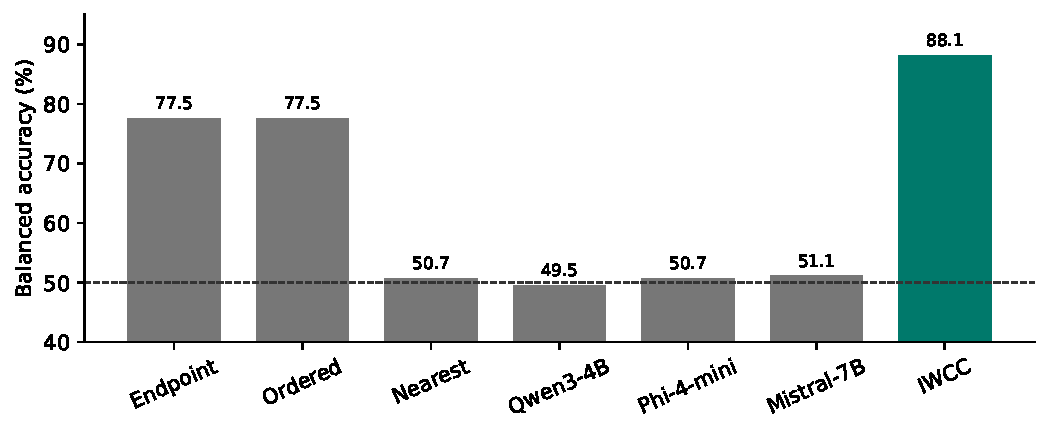
\includegraphics[width=0.98\linewidth]{Fig1.pdf}
\caption{Balanced accuracy on the independent native confirmation. The dashed
line is chance-level balanced accuracy; endpoint-only is the strongest
comparator}
\label{fig:ba}
\end{figure}

\subsection{Environment and operator effects}
\begin{table}[t]
\caption{Balanced accuracy by native environment (percent)}
\label{tab:environment}
\centering
\begin{tabular}{lrrr}
\toprule
Environment & Endpoint & IWCC & Gain \\
\midrule
ALFWorld & 79.39 & 95.61 & 16.23 \\
ScienceWorld & 75.00 & 78.41 & 3.41 \\
\botrule
\end{tabular}
\end{table}

The gain is 16.23 points in ALFWorld and 3.41 points in ScienceWorld. Seven of eight family strata are positive and one is tied; none is negative. The weaker ScienceWorld result is important: IWCC reaches only 78.41\% BA there, and the aggregate claim should not be read as uniformly strong transfer.

Killed-revision recall by operator is 72.55\% for deletion, 74.19\% for adjacent swaps, 80.00\% for truncation, and 76.67\% for role substitution. Endpoint-only detects 0\% of killed adjacent swaps, while IWCC detects 74.19\%, isolating the value of intermediate state/dataflow constraints. Role substitution is not solely responsible for the main effect; the three remaining operators still expose the same mechanism.

\subsection{Auditability and cost}
Among the 154 detected kills, an IWCC violation points exactly to the edited action in 63.64\% and within one action in 94.16\%. The released contract records witness hashes for learned clauses and a canonical content hash. On a single CPU process, 30,000 post-hoc validation calls have median latency \MedianRuntime{} ms and throughput approximately \RuntimeThroughput{} programs/s. In contrast, the three model controls consume 900 GPU inferences and peak at 7.45--13.91 GiB. GPU inference is therefore part of the comparison experiment, not an operational requirement for IWCC.

\section{Discussion}
\subsection{Practical use}
IWCC fits between skill editing and native regression execution. A rejected program can be returned to a developer with a clause and index; an accepted program proceeds to native tests or a risk-limiting release gate. This ordering avoids tool calls for obvious structural defects but preserves native execution as the semantic oracle. Trace hashes let maintainers inspect why a constraint exists and retire it when its witnesses become obsolete.

\subsection{Why endpoint checks fail}
Endpoint rules recognize that a correct goal action appears somewhere. They cannot tell whether the agent reached the corresponding location, still holds the object, or traversed a supported path. Adjacent swaps preserve action vocabulary and often preserve all milestones, which explains the identical endpoint and ordered aggregate results. Abstract state connects producers to consumers and catches these defects without memorizing full traces.

\subsection{Relationship to lifecycle governance}
Contract compilation answers what a skill promises structurally. It does not decide how much native evidence is enough for release, repair a rejected program, or detect conflicts between multiple skills. Those are distinct lifecycle questions. This separation prevents a single artifact from being credited for planning, verification, repair, and governance simultaneously.

\section{Threats to Validity}
\subsection{Construct validity}
Controlled operators are not a sample of naturally occurring skill defects. Role substitutions may be easier than semantic logic errors, while some deleted search actions remain behaviorally irrelevant. Native replay labels address whether each edit actually kills the task, and all survivors are retained, but production-repository evaluation remains necessary.

\subsection{Internal validity}
Development evidence is exposed and supports only method selection. Confirmation task identifiers have zero overlap with prior experiments; source, comparator, prompt, statistics, and gates are hashed before outcomes. The quota-only V2 roster lock is disclosed. Validators never access the private label file, as checked by a released information-boundary audit. Deterministic simulator gold paths limit stochastic variance but do not represent LLM policy variance.

\subsection{External validity}
The study covers two text-based simulators, eight confirmation families, and action programs with parsable commands. It does not cover browser DOM changes, source-code agents, arbitrary shell programs, concurrent skills, hidden permissions, or stochastic external APIs. ScienceWorld's modest gain and the tied non-living family show that trace-backed navigation alone is insufficient for some domains.

\subsection{Statistical validity}
Candidate programs within a task are dependent, so significance is computed on paired task effects and bootstrap resampling is task-stratified. Sixty tasks still give limited family-level precision. The 100,000-draw randomization p-value has a floor near $10^{-5}$. The Wilson intervals are descriptive supplements; the frozen bootstrap of the primary gain drives inference.

\section{Reproducibility}
The artifact releases source, unit tests, both method locks, the zero-overlap roster, 60 healthy trajectories, all 240 mutation specifications and outcomes, public/private candidate separation, 900 model responses, source revisions, hashes, analysis outputs, and both manuscript languages. ALFWorld game files and model weights are referenced by paths/revisions rather than redistributed. Native replay requires the adjacent Paper 01 simulator resources; released-record analysis is CPU-only. The experiment used one RTX 3090 for model controls, Python 3.12, PyTorch 2.8.0, CUDA 12.8, ALFWorld 0.4.2, ScienceWorld 1.2.3, and OpenJDK 17.

\section{Conclusion}
Executable agent skills need more than plausible action lists. IWCC turns successful traces into deterministic, witnessed structural contracts and uses them to screen revisions before execution. On a frozen, zero-overlap ALFWorld/ScienceWorld confirmation, it improves balanced accuracy by \GainPoints{} points over the strongest comparator, with a positive task-clustered interval and no observed false rejection among \ControlCount{} controls. The contribution is intentionally bounded: witnessed contracts expose modeled structural defects cheaply and auditably; native execution remains necessary for unmodeled semantics and real-world reliability.

\backmatter

\section*{Acknowledgements}
The authors have no acknowledgements to report.

\section*{Statements and Declarations}

\subsection*{Funding}
This research received no specific grant from any funding agency in the public,
commercial, or not-for-profit sectors.

\subsection*{Competing interests}
The authors have no relevant financial or non-financial interests to disclose.

\subsection*{Author contributions}
Liang Song: Conceptualization, methodology, software, validation, formal
analysis, investigation, data curation, visualization, writing---original
draft, writing---review and editing, and project administration. Zhai Jiabao:
Methodology, validation, and writing---review and editing. Both authors read
and approved the final manuscript.

\subsection*{Data availability}
The data supporting the findings of this study are included in the frozen
reproducibility package archived in Zenodo at
\url{https://doi.org/10.5281/zenodo.22851666} \citep{song2026iwcc}, with the
public source repository at
\url{https://github.com/ls680/iwcc-agent-skill-contracts}. Third-party ALFWorld
and ScienceWorld assets are not redistributed; pinned upstream revisions,
paths, licenses, and integrity checks are provided instead.

\subsection*{Code availability}
The source code, frozen protocols, analysis scripts, tests, and execution
records are openly available at
\url{https://github.com/ls680/iwcc-agent-skill-contracts} and in the versioned
Zenodo archive at \url{https://doi.org/10.5281/zenodo.22851666}.

\subsection*{Materials availability}
All study-specific materials created by the authors are included in the
reproducibility package. Availability of third-party assets is governed by the
respective upstream projects and licenses.

\subsection*{Ethics approval}
Not applicable. This study evaluates software artifacts and public software
benchmarks and does not involve human participants, animals, clinical data, or
personally identifiable information.

\subsection*{Consent to participate}
Not applicable.

\subsection*{Consent for publication}
Not applicable.

\begin{appendices}
\section{Frozen Confirmation Gates}
The machine-readable summary records all ten criteria individually. No task or outcome is replaced after selection. All model outputs, including uncertain decisions and wrong rejections, remain in the released files. The manuscript is entered in the completion index only because every frozen field is true.

\section{Information Boundary}
The public candidate record has exactly six fields: candidate identifier, environment, family, objective, initial observation, and program. Task locator, variation, operator, edit index, native score, and killed label appear only in the private file opened by the post-hoc analyzer. Source scanning and run specifications attest that all validators keep the private-label flag false.
\end{appendices}

\bibliography{references}

\end{document}
